\begin{wrapfigure}{r}{0.5\textwidth}
  \begin{center}
    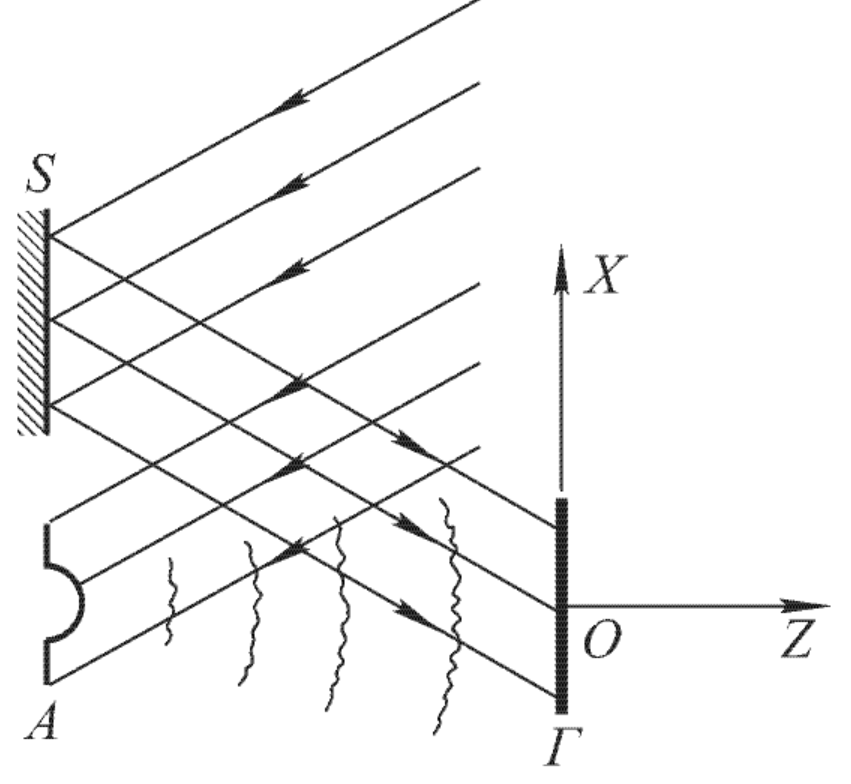
\includegraphics[width=0.28\textwidth]{figures/s54_1.png}
  \end{center}
\end{wrapfigure}
Идея голографии Габора заключается в том, что свет, попадая на объект рассеивается, и рассеянные лучи несут все информацию о форме и рельефе объекта. Однако для восстановления из таких лучей изображения нужна ещё информация о фазе изначально падавшего пучка, которую можно получить, если предварительно разделить этот пучок и часть его пустить на зеркало, чтобы переотразить в область, где мы хотим получать голограмму.
Пучок, рассеивающийся на предмете называется, называется \textit{предметным}, а несущий информацию о фазе -- \textit{опорным}.
Полученная картина на $\Gamma$ записывается, например на чувтсвительную пластину,  и называется голограммой, от греческого <<голог>> -- полный, <<графе>> -- пишу. Позже осветив её той же опорной волной можно получить восстановленное изображение объекта.

Запись голограммы -- очень тонкое дело. Необходимая степень монохроматичности света:
	$\boxed{\frac{\lambda}{\delta l} \gtrsim m}$,
	где $m$ -- максимальный порядок интерференции наблюдающийся при голографировнии.

Для хорошей установки и объекта с линейными размерами $L $ этот порядок можно оценить $\boxed{m \sim \frac{L}{\lambda}}$.
Таким образом должно быть: $\boxed{\delta\lambda < \frac{\lambda^2}{L}}$.

Требования к размеру источника тоже достаточно жестки: $\Delta x = \lambda/\alpha$, где $\alpha$ -- угол схождения крайних интерферирующих лучей. По порядку это что-то вроде $\alpha = h/l$, где $h$ -- ширина опорного пучка, а $l$ -- расстояния между предметом и голограммой. Таким образом $\boxed{\Delta x < \frac{\lambda l}{h}}$.

И так, о чем же сама голография. Представим поле рассеянной волны и отраженной:
\begin{equation*}
	u = a (\vc{r}) e^{i [\omega t - \Phi(\smallvc{r})]},
	\hspace{0.5 cm}
	v = b e^{i (\omega t - \smallvc{k} \smallvc{r})}.
\end{equation*}
Тут мы сделали упрощение, что поля не векторные, а скалярные, что для нас не сильно критично, и при таком упрощении $a(\vc{r})$, $\Phi(\vc{r})$ и $b$ будем считать вещественными. На пластинке $\Gamma$ интенсивность:
\begin{equation*}
	I  = v^* u + v u^* + v^* v + u^* u,
	\hspace{0.5 cm}
	I_0 = b a (x,y,0) e^{i[k_x x - \Phi(x,y,0)]} + b a (x,y,0) e^{-i[k_x x - \Phi(x,y,0)]} + b^2 + a^2(x,y,0).
\end{equation*}
где мы направили ось $Z$ перпендикулярно плоскости $\Gamma = XY$.

Допустим теперь, что нашу пластину, покрытую фотоэмульсией мы проявили и \href{https://youtu.be/y-MyaUcMkhs?t=252}{скопировали}, получив позитив голограммы. Пусть у позитива пропускаемость $D = I_0$, такую позитивную голограмму можно использовать для восстановления $u(\vc{r},t)$.
Для этого голограмму просвечивают таким же $v(\vc{r},t)$, он испытает дифракцию на голограмме типа как на диф-решетке. По методу Рэлея получим поле на выходе и будем искать решение волнового уравнения:
\begin{equation*}
	E_{\text{вых}} = D v (x,y,0) = I_{0} b e^{i (\omega t - k_x x)},
	\hspace{1 cm}
	\frac{\partial^2 E}{\partial x^2} + \frac{\partial^2 E}{\partial y^2} + \frac{\partial^2 E}{\partial z^2} + k^2 E = 0.
\end{equation*}
Будем искать решение для $E$ в виде $E = E_1 + E_2 + E_3 + E_4$, с граничными условиями:
\begin{equation*}
	\begin{aligned}
		&E_{1 \text{ вых}} = b^2 a(x,y,0) e^{i [\omega t - \Phi(x,y,0)]},\\
		&E_{2 \text{ вых}} = b^2 a(x,y,0) e^{i [\omega t + \Phi(x,y,0) - 2 k_x x]},	
	\end{aligned}
	\hspace{1 cm}
	\begin{aligned}
		&E_{3 \text{ вых}} = b^3 e^{i (\omega t - k_x x)},\\
		&E_{4 \text{ вых}} = b a^2(x,y,0) e^{i (\omega t - k_x x)}.
	\end{aligned}
\end{equation*}
Будем решать. Проще всего найти функцию $E_3 = b^3 e^{i (\omega t - \smallvc{k} \smallvc{r})} = b^2 v(\vc{r},t)$, это есть ни что иное, как опорная волна, распространяющаяся за голограмму.

Основной же интерес для голографии представляет собой поле $E_1$, $b$ -- постоянно, тогда:
\begin{equation*}
	E_1 = b^2 a (x,y,z) e^{i [\omega t - \Phi(x,y,z)]} = b^2 u (\vc{r},t).
\end{equation*}
Действительно, видим, что это волна, уходящая от голограммы. Она даст мнимое изображение объекта, в том же самом месте, в котором он находился до получения голограммы. 

Для нахождения $E_2$ сначала посмотрим на случай, когда опорный луч падает нормально плоскости голограммы, тогда $k_x = 0$, и немного другое граничное условие дадут решение
\begin{equation*}
	E_{2 \text{ вых}} = b^2 a(x,y,0) e^{i[\omega t + \Phi(x,y,0)]}
	\hspace{1 cm}
	\Rightarrow
	\hspace{1 cm}
	\tilde{E}_2 (x,y,z) = b^2 a (x,y,z) e^{i [\omega t + \Phi(x,y,z)]}.
\end{equation*}
Такая волна снова создаёт мнимое изображение, как и только что рассмотренная выше $E_1$, но она распространяется к голограмме, а не от нее, значит не может служить решением рассматриваемой нами задачи.
Чтобы починиться в уравнении Гельмгольца заменим $z \mapsto -z$
\begin{equation*}
	\frac{\partial^2 E}{\partial x^2} + \frac{\partial^2 E}{\partial y^2} + \frac{\partial^2 E}{\partial (-z)^2} + k^2 E = 0
	\hspace{1 cm}
	\Rightarrow
	\hspace{1 cm}
	E_2 = b^2 a(x,y,-z) e^{i[\omega t + \Phi(x,y,-z)]}.
\end{equation*}
Теперь волна идёт от голограммы, является решением нашей краевой задачи, и формирует таким образом действительное изображение.